\documentclass[a4paper, 11pt,table]{article}

\usepackage[utf8]{inputenc}
\usepackage[T1]{fontenc}
\usepackage[toc,page]{appendix}
\usepackage{varioref}
\usepackage{hyperref}
\usepackage[nameinlink]{cleveref}
\usepackage{nameref}
\usepackage{parskip}
\usepackage{multicol}%multi column bib
\usepackage[sectionbib, tocbib, numberedbib, bibnewpage]{apacite}%Citations
\usepackage{tikz}
\usepackage{pdflscape}
\usepackage{tabu}
\usepackage{pgfplots}
\usepackage[margin=0.5in]{geometry}

\usepackage{comment}
%\excludecomment{figure}
%\let\endfigure\relax

\pagenumbering{gobble}

\author{Steven Lowes}
\title{Software Methodologies AI Search}
\date{\today{}}

\newcommand{\smartref}[1]{%
	\hyperref[#1]{\cref{#1}, ``\nameref{#1}", \vpageref{#1}}%
}

\begin{document}
	
	\section{Algorithm A: Simulated Annealing}

	\subsection{Description}
	\begin{tabu}{X X[c]}
		Simulated annealing is similar to a hill climbing algorithm, except it will occasionally move down the hill. The chance of doing so decreases as the algorithm nears completion.
		
		Each potential next state is selected with chance
		
		\begin{equation}
		e^{-(newValue - currentValue) / temperature}
		\end{equation}
		
		Temperature is set with a parameter at the start of the algorithm, and decreases exponentially until it reaches the end temperature, also set by a parameter. The rate of decrease is set by another parameter, called cooling rate. After each step the temperature is multiplied by the cooling rate.
		&
		\rowcolors{0}{gray!25}{white}
		\begin{tabu}{|c c|}\hline
			\textbf{Nodes} & \textbf{Tour Length} \\
			12 & 56.0 \\
			17 & 1,514 \\
			21 & 2,668 \\
			26 & 1,479 \\
			42 & 1,217 \\
			48 & 13,999 \\
			58 & 26,740 \\
			175 & 21,519 \\
			180 & 2,540 \\
			535 & 49,007 \\\hline
		\end{tabu}
	
		\vspace{6pt}
		Simulated Annealing Results
	\end{tabu}
		
	\subsection{Start/End Temp}
	When the Start Temperature is too high, the simulation will frequently jump to worse states in the beginning. This means that the algorithm does not even begin to converge until it is a significant way through, wasting lots of computation. If the starting temperature is too low, then the algorithm will get stuck in local minima.
	
	When the End Temperature is very low, the algorithm will spend a long time in a local minima, looking for a better result without ever jumping to a worse result, wasting computation time. If the End Temperature is too high, it will never properly descend into the local minima.
	
	In each test, the cooling rate was set so that the number of steps remained at 1,000,000. This was a deliberately low number of steps, so that the effects of changing the start and end temperatures were exaggerated.
	
			
	\begin{tabu}{X[c] X[c]}		
		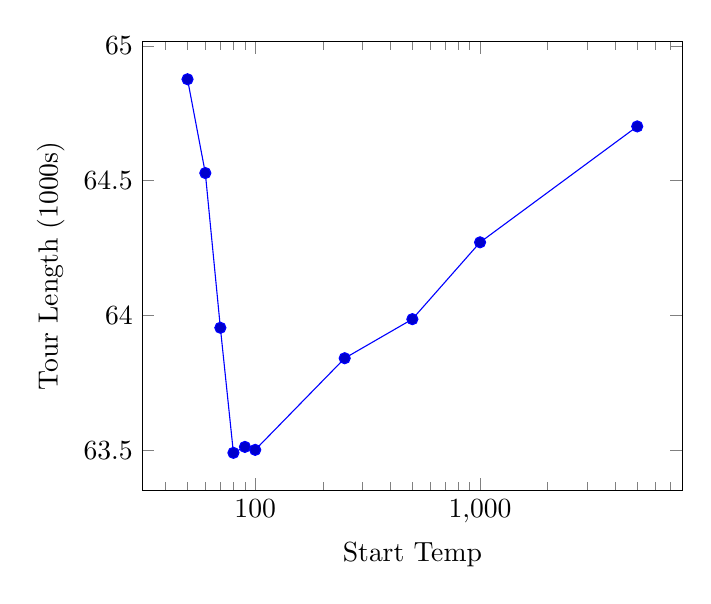
\begin{tikzpicture}
		\begin{axis}[
		%title = Effects of changing start temp,
		xlabel = {Start Temp},
		ylabel = {Tour Length (1000s)},
		xmode=log,
		log ticks with fixed point,
		]
		\addplot coordinates {
			(50,64.876)
			(60,64.528)
			(70,63.954)
			(80,63.490)
			(90,63.512)
			(100,63.501)
			(250,63.841)
			(500,63.986)
			(1000,64.271)
			(5000,64.701)
		};
		\end{axis}
		\end{tikzpicture}&
		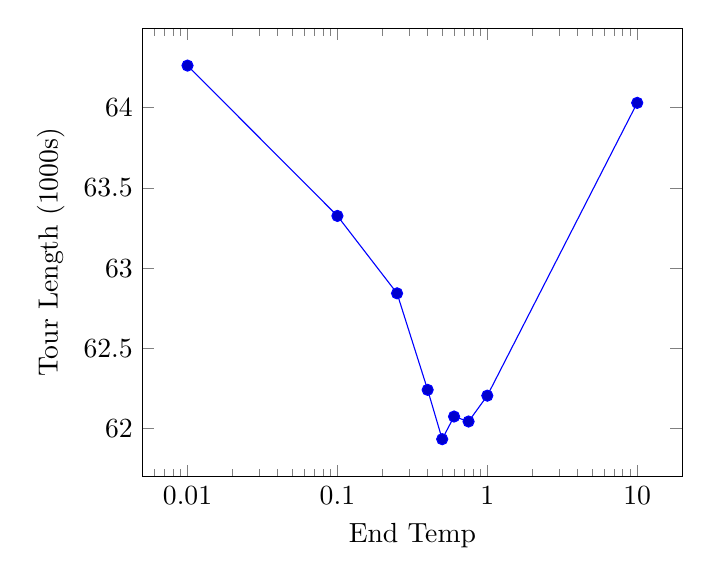
\begin{tikzpicture}
		\begin{axis}[
		%title = Effects of changing end temp,
		xlabel = {End Temp},
		ylabel = {Tour Length (1000s)},
		xmode=log,
		log ticks with fixed point,
		]
		\addplot coordinates {
			(0.01,64.261)
			(0.1,63.325)
			(0.25,62.843)
			(0.4,62.242)
			(0.5,61.935)
			(0.6,62.076)
			(0.75,62.045)
			(1,62.206)
			(10,64.029)
		};
		\end{axis}
		\end{tikzpicture}
	\end{tabu}


\subsection{Multithreading}
Multithreading was implemented into my Simulated Annealing Algorithm. However, I never found a way to make it viable as a way to improve speed while keeping the results of equal quality. The way that I implemented multithreading was to run the simulation in `stages'. Each stage ran the same as the normal simulation, but with the number of steps split between the threads. The stage was run simulatenously on multiple threads. After $x$ steps were complete, the best result found from any of the stages was taken as the new best result, and the temperature updated.

This meant that if $x$ was set too high, then the simulation would be very coarse. If it was set too low, then there would be a very large overhead from creating and destroying new threads. I was not able to find a value in the middle which sped up computation while keeping results of the same quality, or even close. It was quicker just to run the simulation on a single thread but with a quicker cooling rate, and you get results that are equally bad.

On simulations which take weeks, it would probably make sense to enable this method of multithreading. You could set a very high $x$ value, and still get good results. This is becuase the overhead of generating the threads reduces as $x$ increases, but the negative effects on the results is proportional to $steps/x$.

You can show that this method is flawed through \emph{reductio ad absurdum}. Increase the number of steps between each sync to be equal to the $n/cpus$ where $n$ is the total number of steps. Essentially, this method must reduce the quality of results because the alternative is that running annealing 10 times and taking the best result is just as good as running it once with 10 times as many steps.

\subsection{Cooling Rate}
The cooling rate can be changed via a parameter. The cooling rate is equal to $1-f$ where $f$ is the factor by which the temperature is multiplied by after each iteration. High cooling rates means that the simulation runs quicker but more coarsely, producing worse results. Conversely, low cooling rate means that the simulation takes more time, but produces better results. Runtime scales linearly with the number of steps.

\begin{tabu}{X[c] X[c]}
		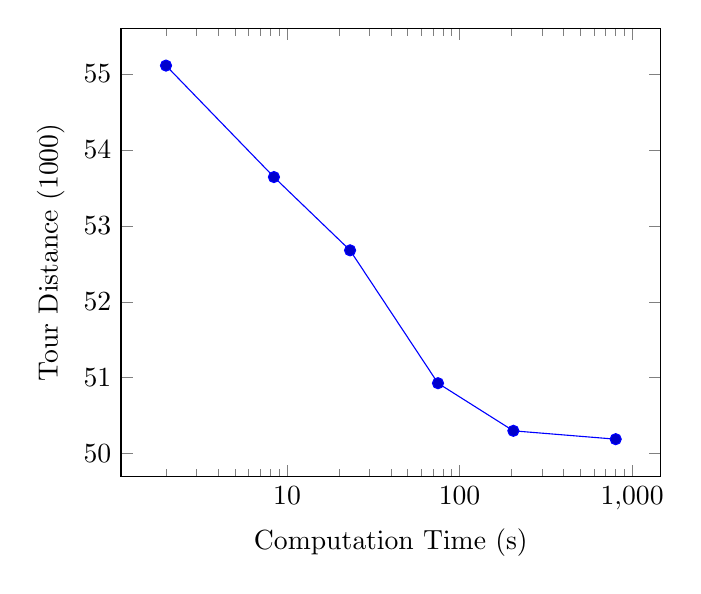
\begin{tikzpicture}
		\begin{axis}[
		%title = Effects of allowing extra computation time,
		xlabel = {Computation Time (s)},
		ylabel = {Tour Distance (1000)},
		xmode=log,
		log ticks with fixed point,
		]
		\addplot coordinates {
			(1.99,55.111)
			(8.40,53.643)
			(23.2,52.678)
			(75,50.928)
			(205,50.301)
			(803,50.191)
		};
		\end{axis}
		\end{tikzpicture}&
		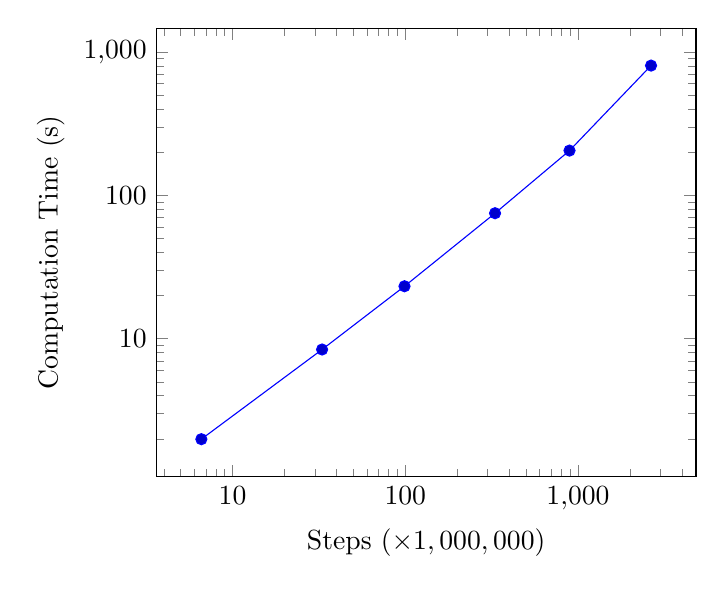
\begin{tikzpicture}
		\begin{axis}[
		%title = Linear time/steps,
		xlabel = {Steps ($\times 1,000,000$)},
		ylabel = {Computation Time (s)},
		xmode=log,
		ymode=log,
		log ticks with fixed point,
		]
		\addplot coordinates {
			(6.6,1.99)
			(33,8.40)
			(99,23.2)
			(331,75)
			(893,205)
			(2648,803)
		};
		\end{axis}
		\end{tikzpicture}
\end{tabu}

\section{Algorithm B: Ant Colony Optimisation}

\subsection{Description}
\begin{tabu}{X X[c]}
	Ant Colony Optimisation simulates a number of ants moving around the graph. At each junction the ant chooses an edge to travel down using a weighted random selection. The weights for each edge are 
	
	\begin{equation}
	Pheromones^{2}*Length^{-2}
	\end{equation}
	
	 Shorter edges are more desirable, as are edges with more pheromones. After each iteration, all ants deposit pheromones on the paths they travelled down. Pheromones then evaporate, with the pheromones on each edge being multiplied by a constant factor.
	&
	\rowcolors{0}{gray!25}{white}
	\begin{tabu}{|c c|}\hline
		\textbf{Nodes} & \textbf{Tour Length} \\
		12 & 56.0 \\
		17 & 1,444 \\
		21 & 2,549 \\
		26 & 1,575 \\
		42 & 1,322 \\
		48 & 12,702 \\
		58 & 25,855 \\
		175 & 21,770 \\
		180 & 1,950 \\
		535 & 50,124 \\\hline
	\end{tabu}
	
	\vspace{6pt}
	Ant Colony Results
\end{tabu}

\subsection{Elite Ant}
In each iteration, the best all-time ant was added to the ants to be processed. This means that the best all-time path has pheremones deposited onto it after each iteration, even if none of the generated ants chose that path.

The algorithm with the Elite Ant consistently outperforms the algorithm without the Elite Ant, albeit marginally. The Elite Ant algorithm ranges from slightly faster to much faster, with tour lengths almost identical.

\begin{tabu}{X[c] X[c]}
	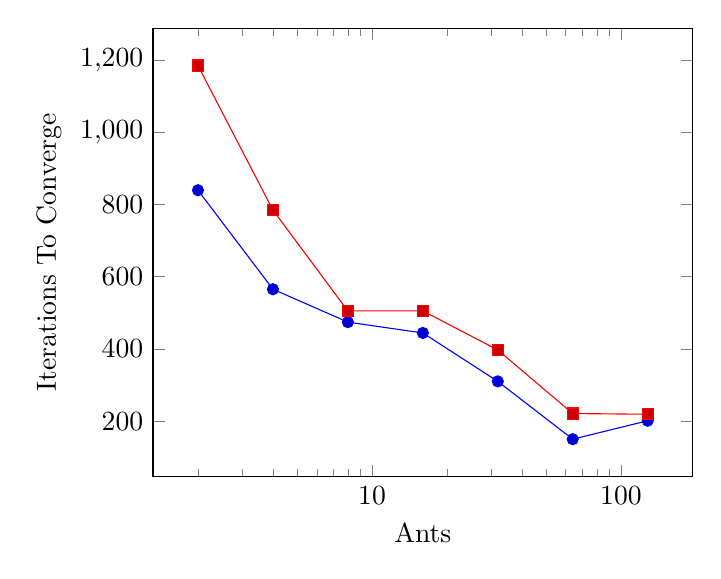
\begin{tikzpicture}
	\begin{axis}[
	%title = Iterations to Converge,
	xlabel = {Ants},
	ylabel = {Iterations To Converge},
	xmode=log,
	log ticks with fixed point,
	]
	\addplot coordinates { %Elite
		(2,839)
		(4,565)
		(8,474)
		(16,444)
		(32,310)
		(64,150)
		(128,201)
	};
	
	\addplot coordinates { %Without
		(2,1184)
		(4,784)
		(8,505)
		(16,505)
		(32,397)
		(64,221)
		(128,219)
	};
	\end{axis}
	\end{tikzpicture}&
	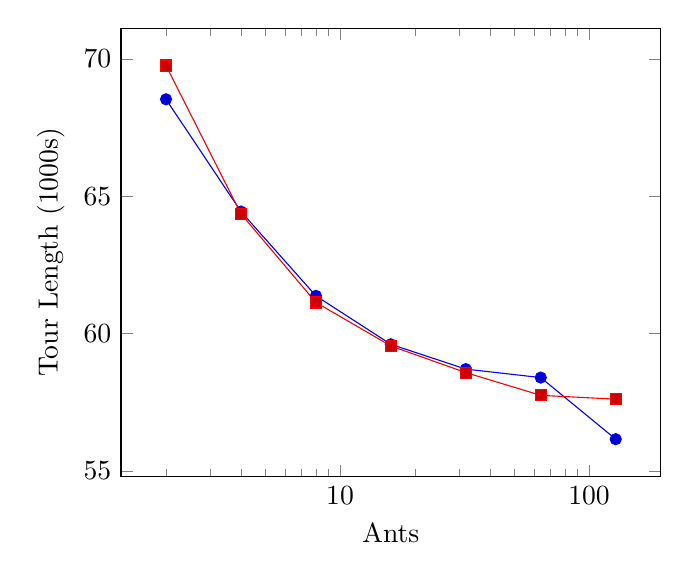
\begin{tikzpicture}
	\begin{axis}[
	%title = Tour Lengths,
	xlabel = {Ants},
	ylabel = {Tour Length (1000s)},
	xmode=log,
	log ticks with fixed point,
	]
	\addplot coordinates { %Elite
		(2,68.531)
		(4,64.445)
		(8,61.375)
		(16,59.612)
		(32,58.710)
		(64,58.401)
		(128,56.159)
	};
	
	\addplot coordinates { %Without
		(2,69.758)
		(4,64.362)
		(8,61.137)
		(16,59.553)
		(32,58.582)
		(64,57.755)
		(128,57.615)
	};
	\end{axis}
	\end{tikzpicture}
\end{tabu}
\vspace{-1cm}
\subsection{Multithreading}
\begin{tabu}{X[c] X[c]}	
	\begin{minipage}{\linewidth}
		Implementing multithreading into the ant colony optimisation was very easy and does not reduce the quality of the results whatsoever. When generating the ant population, create multiple threads and ask each thread to create a portion of the ants. We then combine the generated lists and process the ants in a single-threaded manner.\\
		
		This works due to the fact that the during the generation of the ants, the shared resources are processed in an entirely read-only fashion. The processing step could be run in parallel in future but this will be more difficult to implement due to shared resources being mutated.
	\end{minipage}
	
	&
	\begin{minipage}{\linewidth}
	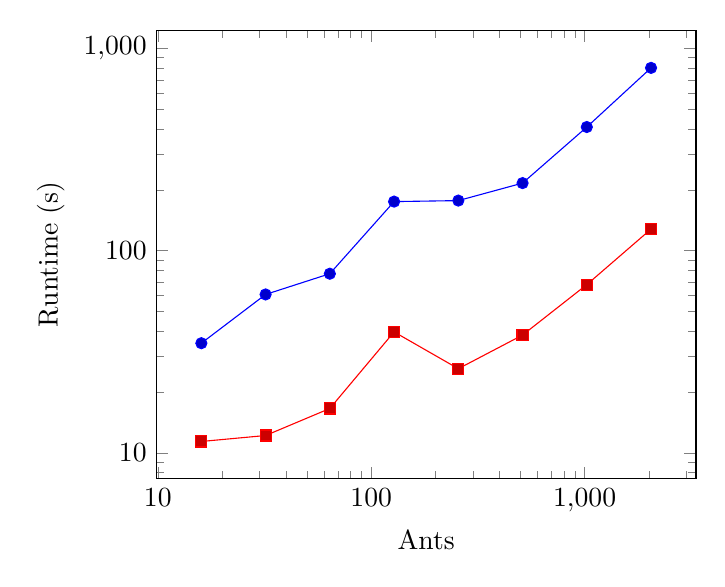
\begin{tikzpicture}
		\begin{axis}[
		xlabel = {Ants},
		ylabel = {Runtime (s)},
		xmode=log,
		ymode=log,
		log ticks with fixed point,
		]
		\addplot coordinates { %ST
			(16,34.9)
			(32,60.8)
			(64,77)
			(128,175)
			(256,177)
			(512,216)
			(1024,409)
			(2048,802)
		};
		
		\addplot coordinates { %MT
			(16,11.4)
			(32,12.2)
			(64,16.6)
			(128,39.7)
			(256,26.1)
			(512,38.3)
			(1024,68)
			(2048,128)
		};
		\end{axis}
	\end{tikzpicture}
	\end{minipage}
	\\
\end{tabu}


\subsection{Culling}
\begin{tabu}{X[c] X[c]}
	\begin{minipage}{\linewidth}
I attempted to improve performance of the ant colony optimisation by culling edges with sufficiently low desirability. This would mean that culled edges did not need to be considered when performing the weighted random selection.\\

However, there was not a happy medium between having the culling happen to early (and therefore reduce the quality of the results) and having it happen too late (by which point the algorithm had already converged and we could have just ended it immediately).
	\end{minipage}&

\begin{minipage}{\linewidth}
	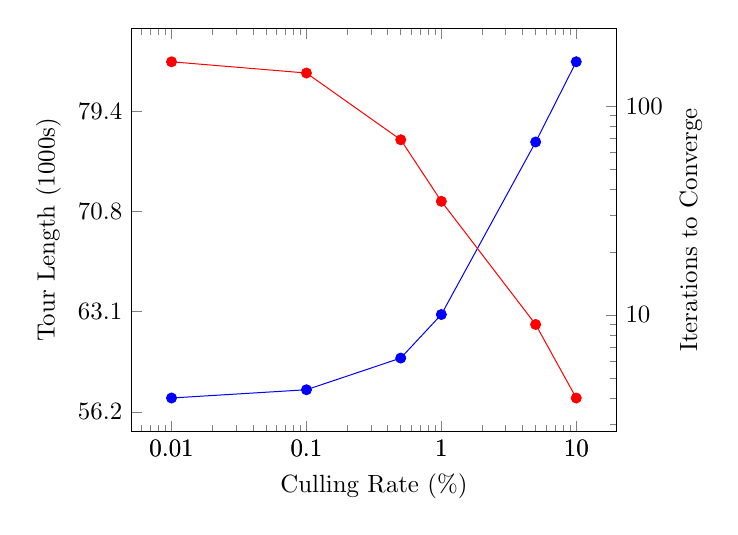
\begin{tikzpicture}[scale=0.9]
	\begin{axis}[
	xlabel = {Culling Rate (\%)},
	ylabel = {Tour Length (1000s)},
	axis y line*=left,
	ylabel near ticks,
	xmode=log,
	ymode=log,
	log ticks with fixed point,
	]
	\addplot[blue,mark=*] coordinates {
		(0.01,57.154)
		(0.1,57.700)
		(0.5,59.838)
		(1,62.910)
		(5,76.699)
		(10,84.099)
	};
	\end{axis}
	
	\begin{axis}[
	ylabel = {Iterations to Converge},
	axis y line*=right,
	ylabel near ticks,
	xmode=log,
	ymode=log,
	log ticks with fixed point,
	]
	\addplot[red,mark=*] coordinates { %ST
		(0.01,163)
		(0.1,144)
		(0.5,69)
		(1,35)
		(5,9)
		(10,4)
	};
	\end{axis}
	\end{tikzpicture}
\end{minipage}
\end{tabu}

\section{General}

\subsection{Fast Triangular Array}
The original way that I stored the matrix was using a HashMap of unordered pairs. This was incredibly slow. Accessing the length of an edge meant creating a new object, hashing it, then retrieving that from the hashtable. I change my approach, creating an array of $size=nodes^2$. When requesting position $(x,y)$, it retrieved position $x_2 \times nodes + y_2$ where $x_2$ was $min(x,y)$ and $y_2$ was $max(x,y)$. This reflects the graph's directionless nature.

\subsection{Grouping}
\begin{tabu}{X[c] X[c]}
	\begin{minipage}{\linewidth}
If we group nodes that are close to each other into groups, we can treat each group as a node in a new network. From here, we can solve the new network, and then solve each group. This can be done recursively --- we can multiple layers of grouping. This technique can produce an approximate solution very quickly, but adding more computation time does not generally improve the results.\\

Choosing how to group the nodes is the main challenge with this technique. This problem is much easier if the network exists in euclidean space. The method selected involved iteratively expanding the group from a start node, in each iteration adding the node with the lowest equivalent electrical resistance to the start node.\\

When treating the groups as nodes, calculating the distances between the nodes is also challenging. If they do not accurately represent how easy it is to move from one group to the other, then the intra-group algorithm will not be efficient. As we progress towards having many levels, these problems are exacerbated. I calculated the new distances to be equal to the average distance between nodes in the two groups.

Once the groups have been generated, each group can be solved in a separate thread, without affecting results whatsoever. The ability to parallelise this algorithm is not particularly helpful, as adding more computation time does not increase the quality of the results much.\\

This approach isn't optimised at all yet, and it wouldn't take much of an improvement in score for this to have a huge impact. The grouping algorithm could be very useful when working with graphs of millions of nodes. Preliminary testing on a graph of 3000 nodes showed this algorithm outperforming plain Simulated Annealing until over 1.5 seconds of computation time was allocated, as opposed to 0.5 seconds on 535 nodes.

	\end{minipage}&

\begin{minipage}{\linewidth}
	\begin{center}
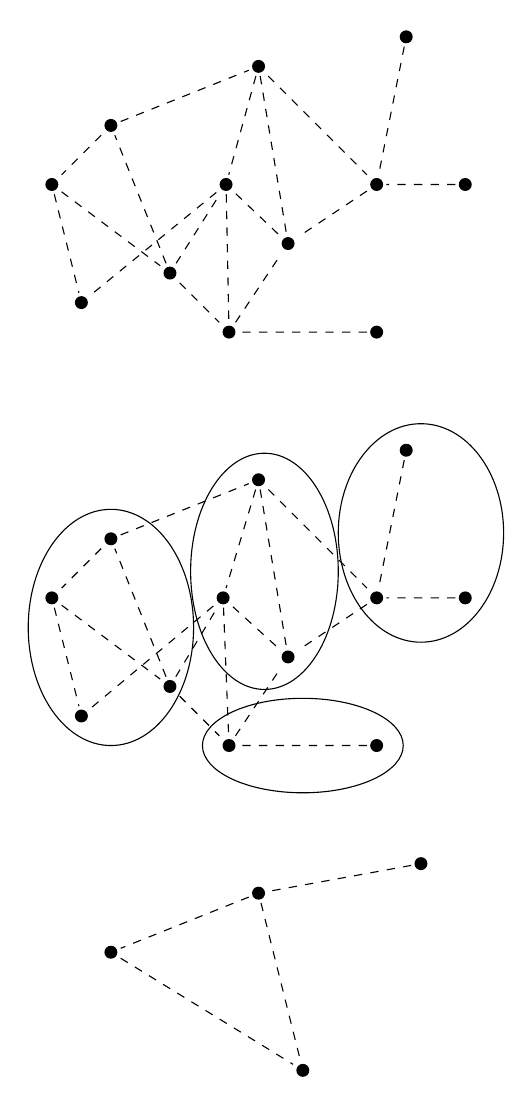
\begin{tikzpicture}[rotate=180,scale=0.75]
\node (v4) at (-4,-20.5) {};
\node (v5) at (-4.95,-22) {};
\node (v7) at (-2,-22) {};
\node (v8) at (-2.5,-20) {};
\node (v6) at (-3,-23) {};
\node (v2) at (-5,-19.5) {};
\node (v11) at (-7.5,-22) {};
\node (v9) at (-5.5,-24) {};
\node (v3) at (-6,-21) {};
\node (v1) at (-7.5,-19.5) {};
\node (v10) at (-8,-24.5) {};
\node (v12) at (-9,-22) {};

\draw (v4) [fill=black] ellipse (0.1 and 0.1);
\draw (v5) [fill=black] ellipse (0.1 and 0.1);
\draw (v7) [fill=black] ellipse (0.1 and 0.1);
\draw (v8) [fill=black] ellipse (0.1 and 0.1);
\draw (v6) [fill=black] ellipse (0.1 and 0.1);
\draw (v2) [fill=black] ellipse (0.1 and 0.1);
\draw (v11) [fill=black] ellipse (0.1 and 0.1);
\draw (v9) [fill=black] ellipse (0.1 and 0.1);
\draw (v3) [fill=black] ellipse (0.1 and 0.1);
\draw (v1) [fill=black] ellipse (0.1 and 0.1);
\draw (v10) [fill=black] ellipse (0.1 and 0.1);
\draw (v12) [fill=black] ellipse (0.1 and 0.1);

\draw [dashed] (v1) edge (v2);
\draw [dashed] (v2) edge (v3);
\draw [dashed] (v4) edge (v5);
\draw [dashed] (v4) edge (v6);
\draw [dashed] (v7) edge (v8);
\draw [dashed] (v7) edge (v4);
\draw [dashed] (v5) edge (v2);
\draw [dashed] (v4) edge (v2);
\draw [dashed] (v9) edge (v5);
\draw [dashed] (v10) edge (v11);
\draw [dashed] (v12) edge (v11);
\draw [dashed] (v11) edge (v3);
\draw [dashed] (v9) edge (v11);
\draw [dashed] (v6) edge (v7);
\draw [dashed] (v5) edge (v8);
\draw [dashed] (v5) edge (v3);
\draw [dashed] (v9) edge (v3);
\draw [dashed] (v6) edge (v9);

\node (v4) at (-4,-13.5) {};
\node (v5) at (-4.9,-15) {};
\node (v7) at (-2,-15) {};
\node (v8) at (-2.5,-13) {};
\node (v6) at (-3,-16) {};
\node (v2) at (-5,-12.5) {};
\node (v11) at (-7.5,-15) {};
\node (v9) at (-5.5,-17) {};
\node (v3) at (-6,-14) {};
\node (v1) at (-7.5,-12.5) {};
\node (v10) at (-8,-17.5) {};
\node (v12) at (-9,-15) {};

\draw (v4) [fill=black] ellipse (0.1 and 0.1);
\draw (v5) [fill=black] ellipse (0.1 and 0.1);
\draw (v7) [fill=black] ellipse (0.1 and 0.1);
\draw (v8) [fill=black] ellipse (0.1 and 0.1);
\draw (v6) [fill=black] ellipse (0.1 and 0.1);
\draw (v2) [fill=black] ellipse (0.1 and 0.1);
\draw (v11) [fill=black] ellipse (0.1 and 0.1);
\draw (v9) [fill=black] ellipse (0.1 and 0.1);
\draw (v3) [fill=black] ellipse (0.1 and 0.1);
\draw (v1) [fill=black] ellipse (0.1 and 0.1);
\draw (v10) [fill=black] ellipse (0.1 and 0.1);
\draw (v12) [fill=black] ellipse (0.1 and 0.1);

\draw [dashed] (v1) edge (v2);
\draw [dashed] (v2) edge (v3);
\draw [dashed] (v4) edge (v5);
\draw [dashed] (v4) edge (v6);
\draw [dashed] (v7) edge (v8);
\draw [dashed] (v7) edge (v4);
\draw [dashed] (v5) edge (v2);
\draw [dashed] (v4) edge (v2);
\draw [dashed] (v9) edge (v5);
\draw [dashed] (v10) edge (v11);
\draw [dashed] (v12) edge (v11);
\draw [dashed] (v11) edge (v3);
\draw [dashed] (v9) edge (v11);
\draw [dashed] (v6) edge (v7);
\draw [dashed] (v5) edge (v8);
\draw [dashed] (v5) edge (v3);
\draw [dashed] (v9) edge (v3);
\draw [dashed] (v6) edge (v9);
\draw (-8.25,-16.1) node (v21) {} ellipse (1.4 and 1.85);
\draw (-6.25,-12.5) node (v22) {} ellipse (1.7 and 0.8);
\draw (-3,-14.5) node (v24) {} ellipse (1.4 and 2);
\draw (-5.6,-15.45) node (v23) {} ellipse (1.25 and 2);

\node (v13) at (-8.25,-10.5) {};
\node (v14) at (-5.5,-10) {};
\node (v16) at (-3,-9) {};
\node (v15) at (-6.25,-7) {};

\draw (v13) [fill=black] ellipse (0.1 and 0.1);
\draw (v14) [fill=black] ellipse (0.1 and 0.1);
\draw (v16) [fill=black] ellipse (0.1 and 0.1);
\draw (v15) [fill=black] ellipse (0.1 and 0.1);

\draw [dashed] (v13) edge (v14);
\draw [dashed] (v14) edge (v15);
\draw [dashed] (v16) edge (v15);
\draw [dashed] (v14) edge (v16);
\end{tikzpicture}

\vspace{12pt}

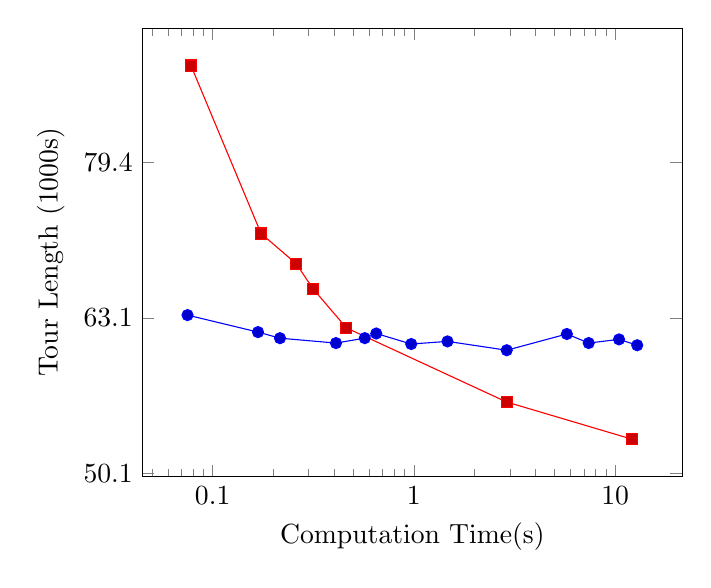
\begin{tikzpicture}
\begin{axis}[
xlabel = {Computation Time(s)},
ylabel = {Tour Length (1000s)},
xmode=log,
ymode=log,
log ticks with fixed point,
]
\addplot coordinates { %Grouping
	(0.075,63.388)
	(0.168,61.811)
	(0.216,61.256)
	(0.41,60.815)
	(0.57,61.262)
	(0.65,61.684)
	(0.97,60.731)
	(1.469,60.966)
	(2.894,60.176)
	(5.759,61.638)
	(7.394,60.822)
	(10.46,61.147)
	(12.88,60.624)
};

\addplot coordinates { %Without
	(0.078,91.704)
	(0.174,71.522)
	(0.26,68.402)
	(0.316,65.884)
	(0.462,62.2)
	(2.89,55.733)
	(12.11,52.753)
};
\end{axis}
\end{tikzpicture}
\end{center}
\end{minipage}
\\
\end{tabu}

\end{document}